
%(BEGIN_QUESTION)
% Copyright 2008, Tony R. Kuphaldt, released under the Creative Commons Attribution License (v 1.0)
% This means you may do almost anything with this work of mine, so long as you give me proper credit

Shown here is a simple schematic diagram for a motor control circuit, using a contactor (``starter'') to switch 3-phase AC power on and off to the motor:

$$\includegraphics[width=15.5cm]{i03623x01.eps}$$

Draw the necessary connecting wires between components to build this circuit:

$$\includegraphics[width=15.5cm]{i03623x02.eps}$$

\vfil

\underbar{file i03623}
\eject
%(END_QUESTION)





%(BEGIN_ANSWER)

This is a graded question -- no answers or hints given!
 
%(END_ANSWER)





%(BEGIN_NOTES)

$$\includegraphics[width=15.5cm]{i03623x03.eps}$$

A helpful hint for circuit sketching, to translate a schematic diagram into a pictorial sketch, is to label the terminals of {\it all} circuit components in order to help identify how to connect them together to form a circuit.  

Here, the only unlabeled device was the toggle switch.  Once the switch's terminals have been labeled on the schematic diagram, and also on the pictorial sketch (before drawing the connecting wires), the wire-sketching becomes a simple matter of ``connect the dots.''

\vskip 10pt

\vskip 20pt \vbox{\hrule \hbox{\strut \vrule{} {\bf Virtual Troubleshooting} \vrule} \hrule}

This question is a good candidate for a ``Virtual Troubleshooting'' exercise.  Presenting the diagram to students, you first imagine in your own mind a particular fault in the system.  Then, you present one or more symptoms of that fault (something noticeable by an operator or other user of the system).  Students then propose various diagnostic tests to perform on this system to identify the nature and location of the fault, as though they were technicians trying to troubleshoot the problem.  Your job is to tell them what the result(s) would be for each of the proposed diagnostic tests, documenting those results where all the students can see.

During and after the exercise, it is good to ask students follow-up questions such as:

\begin{itemize}
\item{} What does the result of the last diagnostic test tell you about the fault?
\item{} Suppose the results of the last diagnostic test were different.  What then would that result tell you about the fault?
\item{} Is the last diagnostic test the best one we could do?
\item{} What would be the ideal order of tests, to diagnose the problem in as few steps as possible?
\end{itemize}

%INDEX% Pictorial circuit review (relay circuit)

%(END_NOTES)


